\documentclass[]{beamer}
%\documentclass[9pt]{beamer}


\mode<presentation>
{
\usetheme{Singapore} %use default if problems or  Singapore or
  % or ... https://deic-web.uab.cat/~iblanes/beamer_gallery/index_by_theme.html
\usefonttheme{serif}
}
\setbeamertemplate{footline}[frame number]
\usepackage{booktabs}
\usepackage{color}

\usepackage[english]{babel}
% or whatever

\usepackage[latin1]{inputenc}
% or whatever

\usepackage{times}
\usepackage[T1]{fontenc}
% Or whatever. Note that the encoding and the font should match. If T1
% does not look nice, try deleting the line with the fontenc.
\usepackage[super]{nth}
\usepackage{xcolor}
\usepackage{relsize} %large math

\usepackage{graphicx} % to insert the logo

\usepackage{hyperref}
\hypersetup{
  colorlinks   = true, %Colours links instead of ugly boxes
  urlcolor     = blue, %Colour for external hyperlinks
  linkcolor    = blue, %Colour of internal links
  citecolor   = red %Colour of citations
}

\usepackage[font=scriptsize,skip=1pt]{caption}

\setbeamertemplate{caption}[numbered]

\title{Uno schema e alcuni link utili}

\author[] % (optional, use only with lots of authors)
{Pietro colpevole \ldots non unico}
% - Give the names in the same order as the appear in the paper.
% - Use the \inst{?} command only if the authors have different
%   affiliation.


\date[] % (optional, should be abbreviation of conference name)
{Rivoli -- 12 febbraio 2022}

\begin{document}

%%%%%%%%%%%%%%%%%%%%%%%%%%%%%%%%%%%%%%%%%%%%%%%%%%%%%%%%%
\begin{frame}


\titlepage


\end{frame}

%%%%%%%%%%%%%%%%%%%%%%%%%%%%%%%%%%%%%%%%%%%%%%%%%%%%%%%%%
\section{Uno schema ABMi}

%%%%%%%%%%%%%%%%%%%%%%%%%%%%%%%%%%%%%%%%%%%%%%%%%%%%%%%%%
\begin{frame}{~} % 1



\begin{figure}[H]
\center
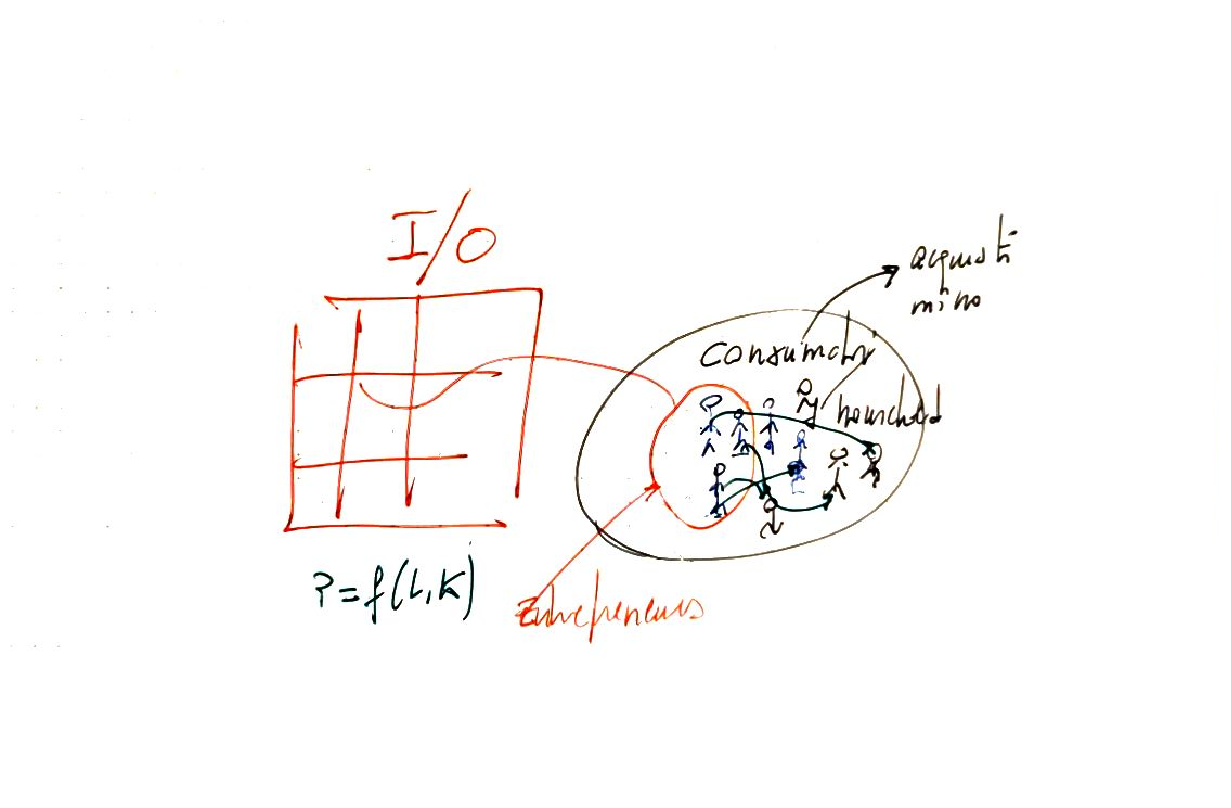
\includegraphics[scale=0.50]{1.pdf}
\label{1}
\caption{Produzione e consumo micro micro}
\end{figure}

\end{frame}

%%%%%%%%%%%%%%%%%%%%%%%%%%%%%%%%%%%%%%%%%%%%%%%%%%%%%%%%%
\begin{frame}{~} % 2



\begin{figure}[H]
\center
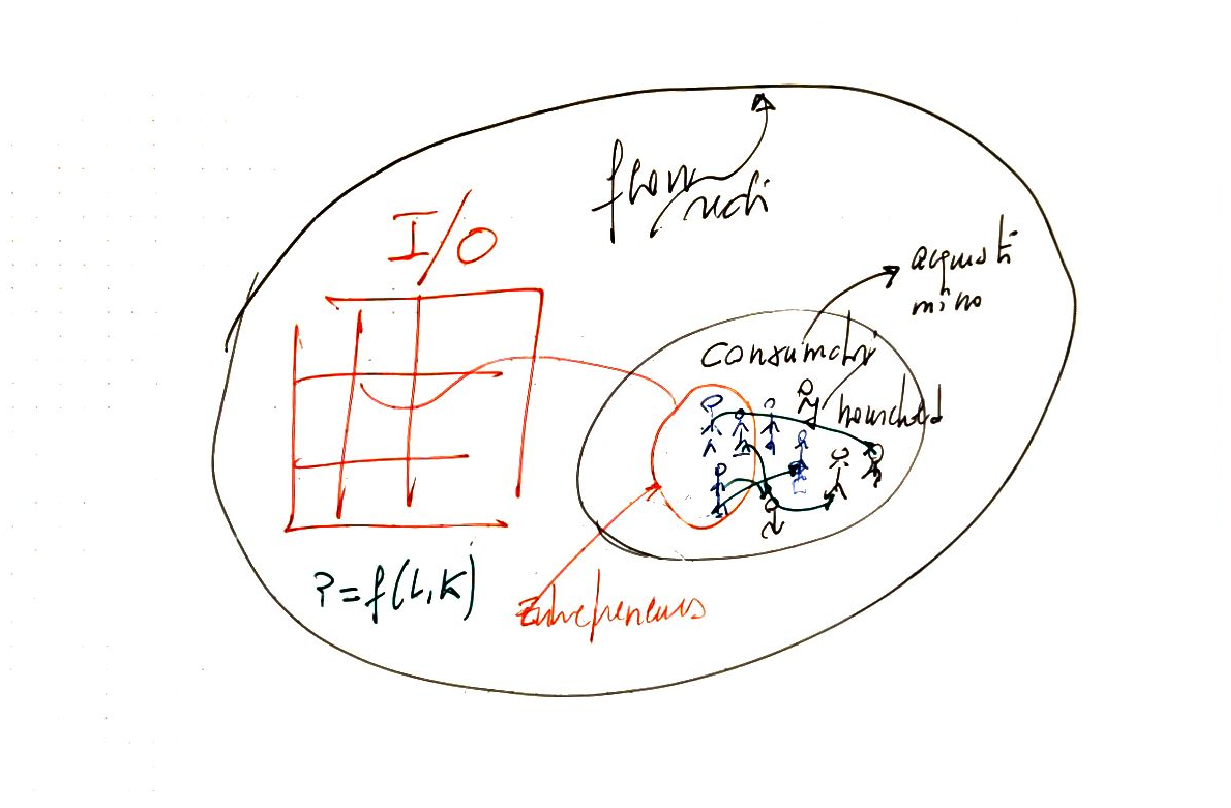
\includegraphics[scale=0.50]{2.pdf}
\label{2}
\caption{Quadratura flussi reali, con produzione, consumi e \ldots}
\end{figure}

\end{frame}

%%%%%%%%%%%%%%%%%%%%%%%%%%%%%%%%%%%%%%%%%%%%%%%%%%%%%%%%%
\begin{frame}{~} % 3



\begin{figure}[H]
\center
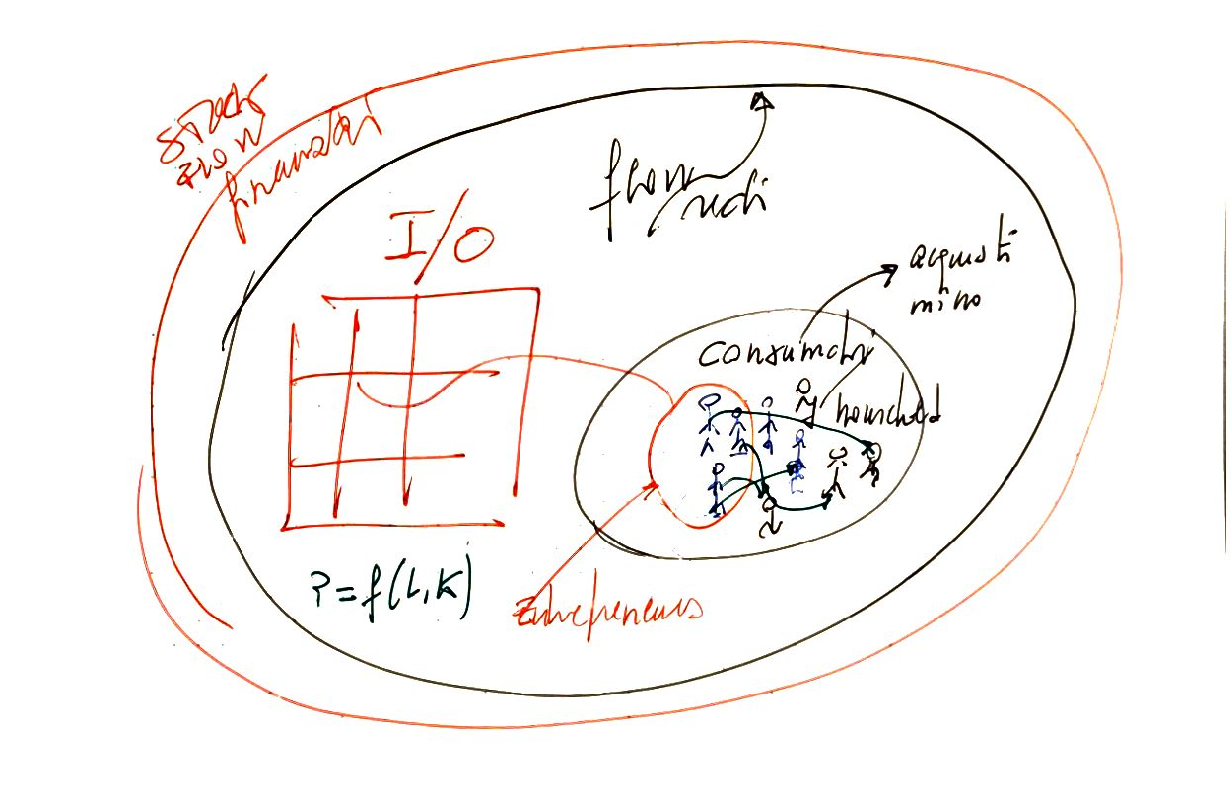
\includegraphics[scale=0.50]{3.pdf}
\label{3}
\caption{Quadratura stock flussi finanziari, con produzione, consumi e \ldots}
\end{figure}

\end{frame}

%%%%%%%%%%%%%%%%%%%%%%%%%%%%%%%%%%%%%%%%%%%%%%%%%%%%%%%%%
\begin{frame}{~} % 4



\begin{figure}[H]
\center
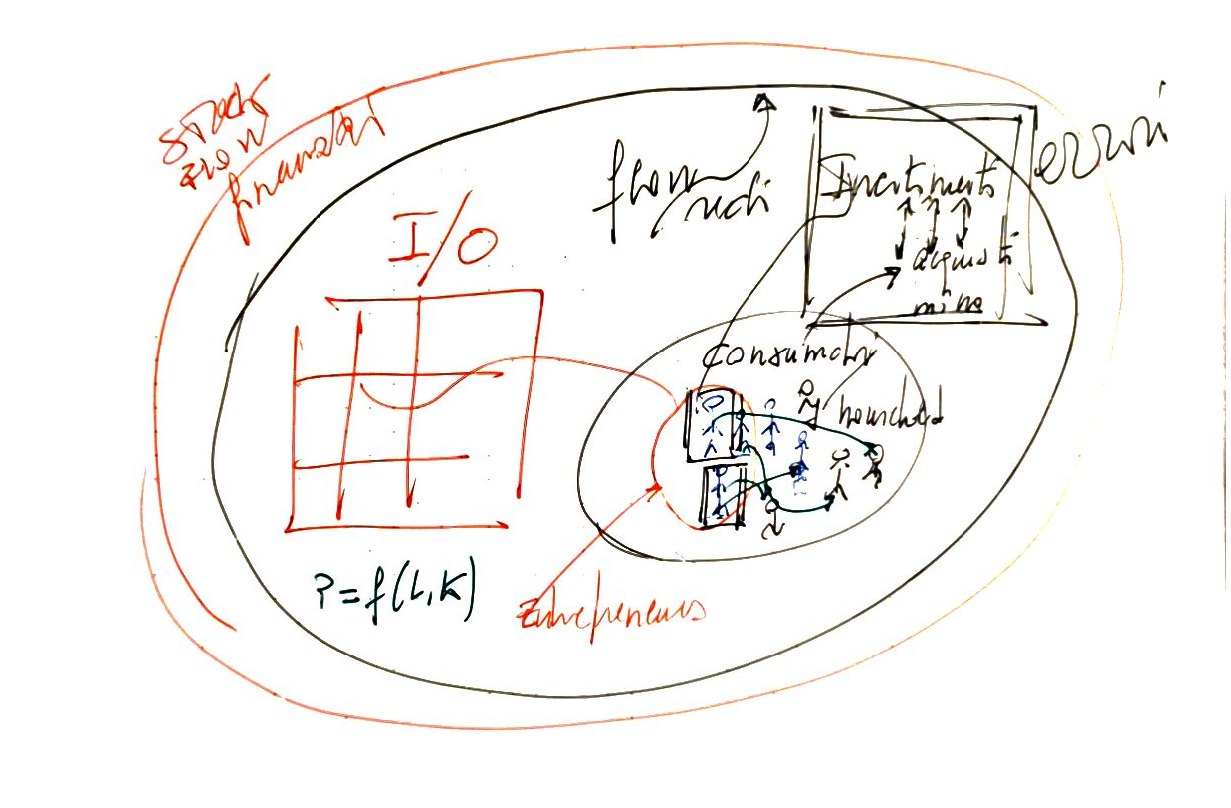
\includegraphics[scale=0.50]{4.pdf}
\label{4}
\caption{\ldots investimenti}
\end{figure}

\end{frame}

%%%%%%%%%%%%%%%%%%%%%%%%%%%%%%%%%%%%%%%%%%%%%%%%%%%%%%%%%
\begin{frame}{~}



\begin{figure}[H]
\center
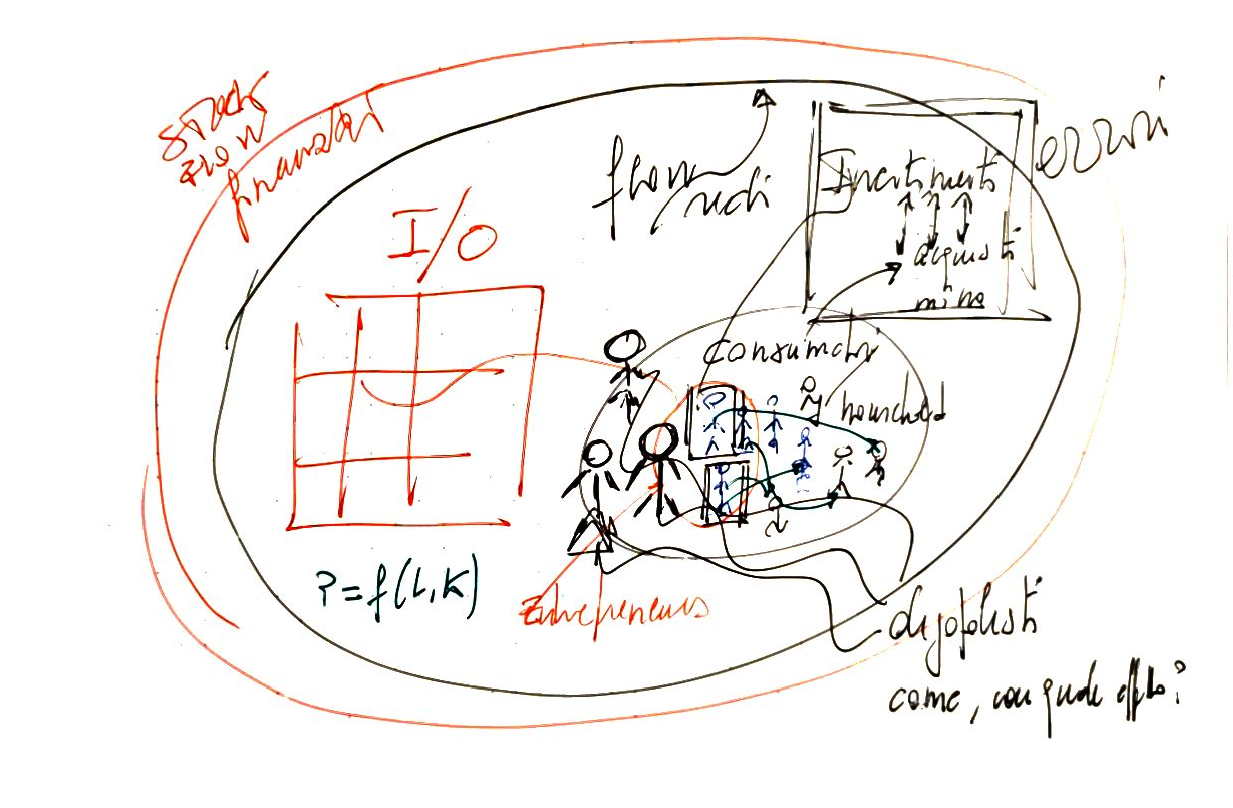
\includegraphics[scale=0.50]{5.pdf}
\label{5}
\caption{Con oligopolisti}
\end{figure}

\end{frame}

%%%%%%%%%%%%%%%%%%%%%%%%%%%%%%%%%%%%%%%%%%%%%%%%%%%%%%%%%
\begin{frame}{~} % 6



\begin{figure}[H]
\center
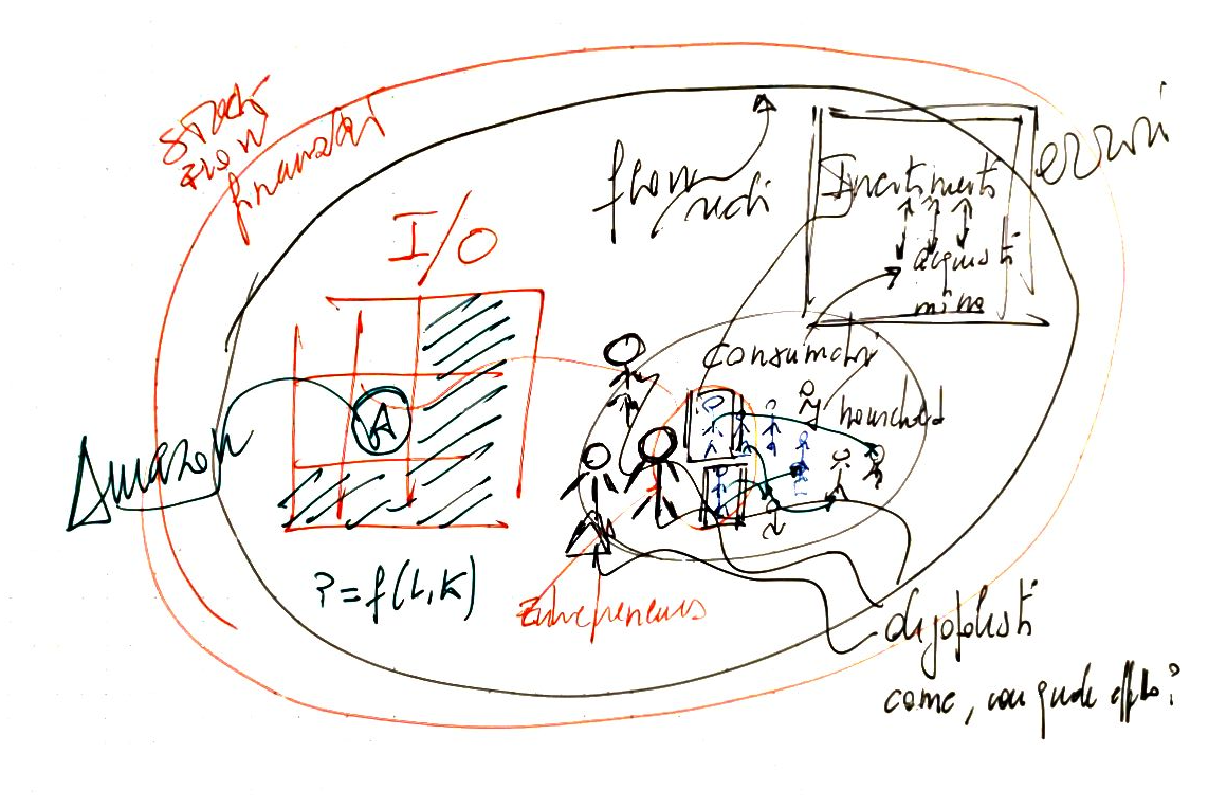
\includegraphics[scale=0.50]{6.pdf}
\caption{Sovrapposizione produzione industriale e commercializzazione e \ldots CHI DECIDE CHE COSA PRODURRE?}
\label{6}
\end{figure}

\end{frame}


%%%%%%%%%%%%%%%%%%%%%%%%%%%%%%%%%%%%%%%%%%%%%%%%%%%%%%%%%
\begin{frame}{~} % 7



\begin{figure}[H]
\center
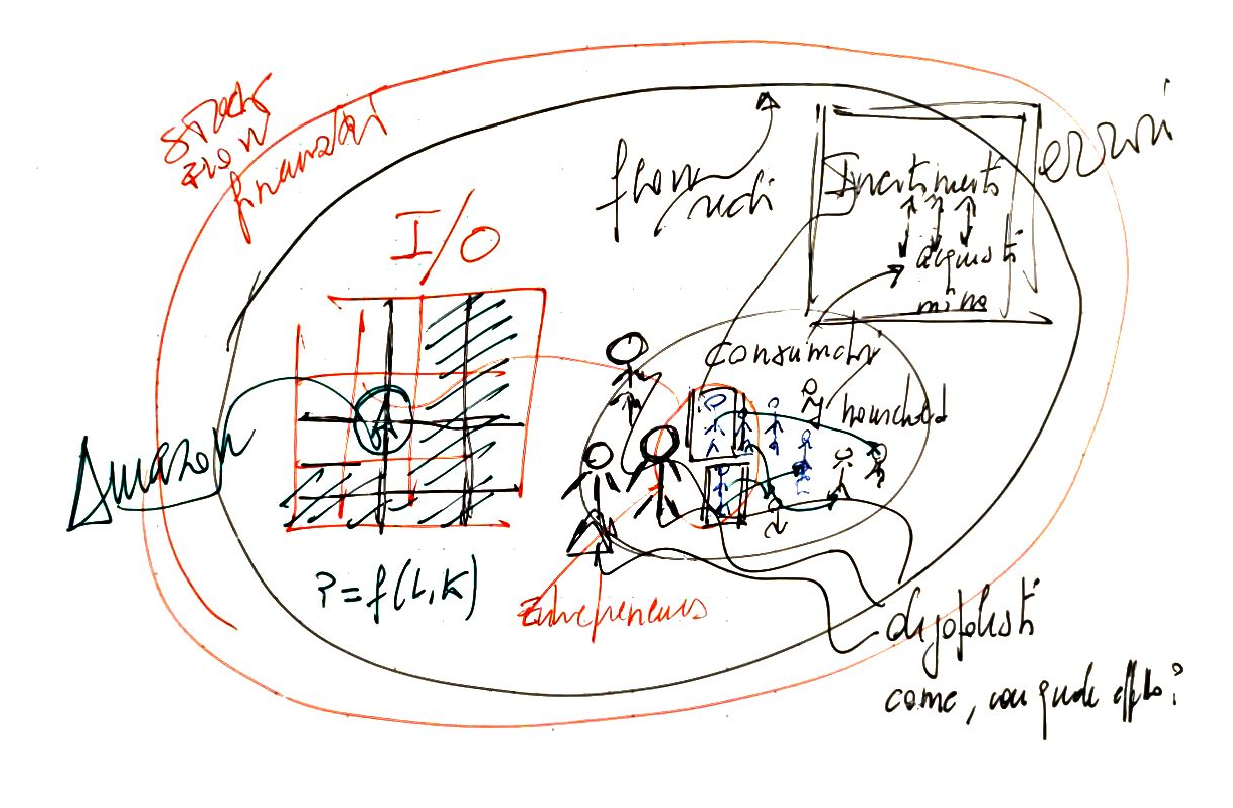
\includegraphics[scale=0.50]{7.pdf}
\label{7}
\caption{Produzione e commercializzazione distinte per beni di consumo e beni investimento}
\end{figure}

\end{frame}

%%%%%%%%%%%%%%%%%%%%%%%%%%%%%%%%%%%%%%%%%%%%%%%%%%%%%%%%%
\section{Linksi}

%%%%%%%%%%%%%%%%%%%%%%%%%%%%%%%%%%%%%%%%%%%%%%%%%%%%%%%%%
\begin{frame}{Queste slide, Overleaf, GitHub, edito formule}

\begin{itemize}

\item
\href{https://terna.to.it/ejmmp/deposito/schemaPietroConLink.pdf}{schemaPietroConLink.pdf}

\item
sta in \href{https://it.overleaf.com/4892961924fddsgrqnbwhh}{Overleaf} con riserva in \href{https://github.com/terna/ejmmpSchemaPietro}{GitHub}

\item
\href{https://editor.codecogs.com}{editor di formule}

\end{itemize}


\end{frame}

%%%%%%%%%%%%%%%%%%%%%%%%%%%%%%%%%%%%%%%%%%%%%%%%%%%%%%%%%
\begin{frame}{Deposito e link}

\href{https://terna.to.it/ejmmp/deposito/}{Deposito}, con:

\begin{itemize}

\item
un importante \href{https://terna.to.it/ejmmp/deposito/stockFlow.pdf}{paper} ABM/stock-flow.

\item
un \href{https://terna.to.it/ejmmp/deposito/JackIonHayek'sEconomics.pdf}{paper} e una \href{https://terna.to.it/ejmmp/deposito/JackIIonHayek-NoteOnAtomicInvestmentProcesses.pdf}{nota} di Jack;

\item
la \href{https://terna.to.it/ejmmp/deposito/MarcoBookProposalTheoreticalModelBookProposal.pdf}{book proposal} di Marco; la nota di Marco si collega al primo modello, del quale abbiamo anche le \href{https://terna.to.it/oligopolyAgentization.pdf}{slide} di una presentazione (eq. \& ABM) che ho fatto a Agentization;

\item
la \href{https://terna.to.it/ejmmp/deposito/PietroBookProposal.pdf}{folle book proposal} di Pietro, cui si collega un \href{https://www.igss-workshop.org}{convegnone} sulla iGSS con la \href{https://www.youtube.com/watch?v=X7DLFvOhqVo}{presentazione} il modello del virus, visibili nelle \href{https://static1.squarespace.com/static/5e0a8466674f5b6963a2e949/t/60bff462ace45c3d0b9f04cf/1623192677563/terna-slides.pdf}{slide};

all'idea di iGGS con Genetic Algorithms collego un micro-modello NetLogo costruito per interagire con gli \emph{ABMgnostic}; \È anche quello nel deposito, come \href{https://terna.to.it/ejmmp/deposito/theRace.zip}{zip}.

\item
J. Doyne Farmer, Simulation conference September 1, 2021, \emph{Simulating the economy
(and the financial system in particular)}, \href{https://www.suomenpankki.fi/globalassets/en/financial-stability/payment-and-settelement-system-simulator/events/2021_01_farmer.pdf}{slide}, con riferimenti all'ambiente.


\end{itemize}

%\href{}{}
\end{frame}

%%%%%%%%%%%%%%%%%%%%%%%%%%%%%%%%%%%%%%%%%%%%%%%%%%%%%%%%%
\begin{frame}{Strumenti}

Che cosa usiamo?

\begin{itemize}

\item
\href{https://terna.github.io/SLAPP/}{SLAPP} oppure \ldots

\item
\href{https://repast.github.io/repast4py.site/index.html}{Repast4Py}?

A giugno, un seminario presso IRES Piemonte su Repast4Py (idea di un modello ABM sul Piemonte, microfondato, stock-flow)

\end{itemize}

Portare in giro lavori preliminari?

\href{https://ssc2022.behavelab.org}{SSC2022} is the 17th annual Social Simulation Conference and will take place from 12--16 September 2022 at the University of Milan, Italy.

\href{https://ssc2022.behavelab.org/submissions/}{Deadline} 15 May 2022.

%\href{}{}
\end{frame}

\end{document}

